
\documentclass{svmult-ddm}

\usepackage{mathptmx}       % selects Times Roman as basic font
\usepackage{helvet}         % selects Helvetica as sans-serif font
\usepackage{courier}        % selects Courier as typewriter font
\usepackage{type1cm}        % activate if the above 3 fonts are
                            % not available on your system
\usepackage{graphicx}        % standard LaTeX graphics tool

                             % when including figure files

\usepackage[bottom]{footmisc}% places footnotes at page bottom

\usepackage{amssymb}
\usepackage{amsfonts}
\usepackage{amsbsy}
\usepackage{amscd}
\usepackage{amstext}
\usepackage{dsfont}
\usepackage[english]{babel}
\usepackage{color}
\usepackage{graphics}
\usepackage{epsfig}
\usepackage{subfigure} 
\usepackage{wrapfig}
\usepackage{psfrag}
\usepackage{color}
\usepackage{url}
\usepackage{verbatim}
\usepackage{algorithm}
\usepackage{algorithmic}

%\usepackage{amsmath}

\begin{document}

\title*{Pipeline Schwarz Waveform Relaxation}
% Use \titlerunning{Short Title} for an abbreviated version of
% your contribution title if the original one is too long
  \titlerunning{Pipeline Schwarz Waveform Relaxation}

\author{Scott High, Pranjal Vachaspati, James Stevens}
%\authorrunning{B.~Ong, S.~High and F.~Kwok}
% Use \authorrunning{Short Title} for an abbreviated version of
% your contribution title if the original one is too long

\maketitle

% \abstract{ To leverage the computational capability of modern
%   supercomputers, existing algorithms need to be reformulated in a
%   manner that allows for many concurrent operations.  In this paper,
%   we outline a framework that reformulates classical Schwarz waveform
%   relaxation so that successive waveform iterates can be computed in a
%   parallel pipeline fashion after an initial start-up cost.  The
%   communication costs for various implementations are discussed, and 
%   numerical scaling results are presented.
% \keywords{
%     Schwarz waveform relaxation, pipeline parallelism, domain
%     decomposition, distributed computing } }


\section{Introduction}
\label{prop_sec:introduction}

Schwarz Waveform Relaxation (SWR), introduced in \cite{bjorhus1995},
is a domain decomposition based method for solving time dependent
PDEs.
% has been analyzed for a wide range of time-dependent problems,
% including the parabolic heat equation \cite{MR1638096}, wave
% equation and advection-diffusion equations
% \cite{gander1999,MR1941398}, Maxwell's equations
% \cite{courvoisier2013}, and the porous medium equation
% \cite{japhet2013}.
In contrast to classical Schwarz iterations, where
the time-dependent PDE is discretized in time and domain-decomposition
is applied to the sequence of steady-state problems, SWR solves {\em
  time-dependent} sub-problems; this relaxes synchronization of the
sub-problems and provides a means to couple disparate solvers applied
to individual sub-problems,
% for example \cite{lemarie:hal-00872496}.
% SWR has also been shown in \cite{MR1941398, MR2448703} to have
% superlinear convergence for small time windows.
Pipeline schwarz waveform relaxation (PSWR), introduced in \cite{ongpipeline},
extends the spatial parallelism of SWR methods to the time domain by
computing successive iterations in a pipeline fashion.
% This paper outlines a framework that
% reformulates SWR so that successive waveform iterates can be computed
% in a pipeline fashion, allowing for increased concurrency and hence,
% increased scalability for SWR-type algorithms.
% In \S\ref{prop_sec:waveform}, we
% review the SWR algorithm before introducing and comparing several
% Pipeline Schwarz Waveform Relaxation algorithms (PSWR) in
% \S\ref{prop_sec:pipeline_waveform}.  Numerical scaling
% results for the linear heat equation are presented in
% \S\ref{prop_sec:numerics}.

\section{Problem Description}
\label{prop_sec:waveform}

Denote the PDE of interest as 
\begin{eqnarray}
  \label{prop_eqn:pde1}
  u_t =  \mathcal{L}(t,u), \quad (x,t)\in \Omega\times[0,T]\\
  \nonumber
  u(x,0) = f(x), \quad x \in \Omega \\
  \nonumber
  u(z,t) = g(z,t), \quad z \in \partial\Omega. 
\end{eqnarray}
Consider a partitioning of the domain, $\Omega = \cup_i\Omega_i$.
The domains in the partition may be overlapping or non-overlapping.
Let $u_i$ denote the solution on sub-domain $\Omega_i$.
Then, equation~(\ref{prop_eqn:pde1}) can be decomposed into a
coupled system of equations,
\begin{eqnarray}
  \label{prop_eqn:pde2}
  (u_i)_t =  \mathcal{L}(t,u_i), \quad (x,t)\in \Omega_i\times[0,T]\\
  \nonumber
  u_i(x,0) = f(x), \quad x \in \Omega_i \\
  \nonumber
  u_i(z,t) = g(z,t), \quad z \in \partial\Omega_i\cap\partial\Omega, \\
  \nonumber
  \mathcal{T}_{ij}(u_{i}(z,t)) = \mathcal{T}_{ij}(u_{j}(z,t)), \quad z \in \partial\Omega_i\cap\partial\Omega_j.
\end{eqnarray}
where $T$ are transmission operators appropriate to the
equation~(\ref{prop_eqn:pde1}).  SWR decouples the system of
PDEs in equation~(\ref{prop_eqn:pde2}).  Let $u_i^{[k]}$
denote the $k$-th waveform iterate on sub-domain $\Omega_i$. After
specifying an initial estimate for the sub-domain solution on the
interfaces, $u_i^{[0]}(z,t),
z\in\partial\Omega_i\setminus\partial\Omega$, the SWR algorithm
iteratively solves PDEs (\ref{prop_eqn:pde3}) for waveform
iterates $k=1,2,\ldots$ until convergence,
\begin{eqnarray}
  \label{prop_eqn:pde3}
  (u_i^{[k]})_t =  \mathcal{L}(t,u_i^{[k]}), \quad (x,t)\in \Omega_i\times[0,T]\\
  \nonumber
  u_i^{[k]}(x,0) = f(x), \quad x \in \Omega_i \\
  \nonumber
  u_i^{[k]}(z,t) = g(z,t), \quad z \in \partial\Omega_i\cap\partial\Omega, \\
  \nonumber
  \mathcal{T}_{ij}(u_{i}^{[k]}(z,t)) = \mathcal{T}_{ij}(u_{j}^{[k-1]}(z,t)), \quad z \in \partial\Omega_i\cap\partial\Omega_j.
\end{eqnarray}

% \begin{table}[htbp]
% \noindent\hrulefill
% {\bf Schwarz Waveform Relaxation Algorithm} 
% \hrulefill \\
% 1. {\tt MPI Initialization}\\
% 2. {\tt parallel for } $i = 1\ldots N$ {\em (Sub-domain)} \\
% 3. \quad\quad {\tt for} $t = \Delta t \ldots T$ \\
% 4. \quad\quad\quad\quad {\tt Guess} $u_i^{[0]}(z,t), \quad z \in \partial\Omega_i\cap\partial\Omega_j$\\
% 5. \quad\quad {\tt end} \\
% 6. {\tt end} \\
% 7. {\tt for } $k=1 \ldots K$ {\em (Waveform iteration)}\\
% 8. \quad\quad {\tt parallel for } $i = 1\ldots N$ {\em (Sub-domain)}\\
% 9. \quad\quad\quad\quad {\tt for} $t = \Delta t \ldots T$ \\
% 10.\quad\quad\quad\quad\quad\quad {\tt Solve for } $u_i^{[k]}(t, x)$ \\
% 11.\quad\quad\quad\quad {\tt end} \\
% 12.\quad\quad\quad\quad {\tt for} $t = \Delta t \ldots T$ \\
% 13.\quad\quad\quad\quad\quad\quad {\tt Exchange transmission data} $\mathcal{T}(u_i^{[k]}(t, z))$ \\
% 14.\quad\quad\quad\quad {\tt end} \\
% 15.\quad\quad\quad\quad {\tt Check convergence} \\
% 16.\quad\quad {\tt end}\\
% 17. {\tt end} \\
% .\hrulefill  \\

% \end{table}
% A pseudo-code for the algorithm is presented on the next page.
% Observe that SWR allows for each sub-domain to independently compute
% time-dependent solutions on their respective sub-domains (lines 9-11)
% During each waveform iteration, transmission data on each sub-domain
% is aggregated for the entire computational time interval before
% boundary data is exchanged between neighboring sub-domains (lines
% 12-14).

% \section{Pipeline Schwarz Waveform Relaxation}
% \label{prop_sec:pipeline_waveform}

Using a similar approach described in
\cite{ChristliebMacdonaldOng2010,MR1340665}, the relaxation framework can be
rewritten so that after initial start-up costs, multiple waveform
iterations can be computed in a pipeline-parallel fashion. A graphical
example of the PSWR algorithm for two subdomains is shown in
Figure~\ref{prop_sec:pswr_fig}.
\begin{figure}
  \centering
  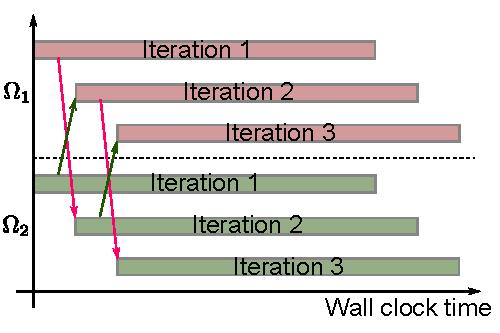
\includegraphics[width=0.5\textwidth]{figure1}
  \caption{The PSWR algorithm allows for multiple Schwarz waveform
    iterations to be simultaneously computed.  After an initial
    start-up cost, multiple iterates are computed in a pipeline
    fashion.}
  \label{prop_sec:pswr_fig}
\end{figure}

The pipelined algorithm has several features that make it an
attractive candidate for implementation in Charm++.  A PSWR iteration
can only proceed if boundary data (i.e. transmission conditions) from
the previous iterates are available; however, any iteration can
proceed for as long as it has updated boundary data regardless of the
current state of the next (or any other) iteration. In the original
MPI implementation, transmission data is exchanged after every time
step, resulting in lock step parallelism. The Charm frameworks ability
to buffer messages and dynamically schedule processes can be used to
relax this tight synchronization, better exploiting the problems
inherent parallelism.


% To simplify
% the presentation, 
%we make the assumption that 
%
% we first present the algorithm for the simplified case where 
% the {\em same} time discretization is used for all sub-problems
%Generalizations to allow for disparate time discretizations for each
%sub-problem are possible, but not discussed here.
% (Pipeline Schwarz Waveform Relaxation Algorithm 1).
% \begin{table}[htbp]
% \noindent\hrulefill
% {\bf Pipeline Schwarz Waveform Relaxation Algorithm 1} 
% \hrulefill \\
% 1. {\tt MPI Initialization}\\
% 2. {\tt parallel for } $i = 1\ldots N$ {\em (Sub-domain)} \\
% 3. \quad\quad {\tt for} $t = \Delta t \ldots T$ \\
% 4. \quad\quad\quad\quad {\tt Guess} $u_i^{[0]}(z,t), \quad z \in \partial\Omega_i\cap\partial\Omega_j$\\
% 5. \quad\quad {\tt end} \\
% 6. \quad\quad {\tt Set} $t^{[0]} = T$\\
% 7. {\tt end} \\
% 8. {\tt parallel for } $k=1 \ldots K$ {\em (Waveform iteration)}\\
% 9. \quad\quad {\tt parallel for } $i = 1\ldots N$ {\em (Sub-domain)}\\
% 10. \quad\quad\quad\quad {\tt set} $t^{[k]} = \Delta t$ \\
% 11. \quad\quad\quad\quad {\tt While} $t^{[k]} \le T$ \\
% 12. \quad\quad\quad\quad\quad\quad {\tt If } $t^{[k]} < t^{[k-1]}$ \\
% 13. \quad\quad\quad\quad\quad\quad\quad\quad {\tt Solve for } $u_i^{[k]}(t^{[k]}, x)$ \\
% 14. \quad\quad\quad\quad\quad\quad\quad\quad {\tt Exchange transmission data} $\mathcal{T}(u_i^{[k]}(t^{[k]}, z))$ \\
% 15. \quad\quad\quad\quad\quad\quad\quad\quad $t^{[k]} \leftarrow t^{[k]} + \Delta t$\\
% 16. \quad\quad\quad\quad\quad\quad {\tt end}\\
% 17. \quad\quad\quad\quad {\tt end} \\
% 18. \quad\quad\quad\quad {\tt Check convergence} \\
% 19. \quad\quad {\tt end}\\
% 20. {\tt end} \\
% .\hrulefill  \\
% \end{table}

% Several observations should be made about the proposed PSWR algorithm.
% First, a Schwarz iteration can only proceed if boundary data
% (i.e. transmission conditions) from the previous iterate are
% available; this condition (part of the start-up cost before the PSWR
% algorithm can be run in a pipeline fashion) is checked by the {\tt if}
% statement in line~12.  Secondly, transmission data is exchanged after
% every time step to facilitate the pipeline parallellism.  This added
% synchronization can be relaxed at the expense of increasing the
% start-up cost needed to run this algorithm in a pipeline fashion.
% This pipeline parallelism allows for $N\cdot K$ concurrent processes
% in the PSWR algorithm with efficiency $\frac{N_t}{K+N_t}$ (accounting
% for start-up costs), where $N_t$ is the number of time steps used to
% discretize the time domain $[0,T]$, $N$ is the number of sub-domains,
% $K$ is the number of waveform iterates.  This contrasts with the SWR
% algorithm, which can only utilize $N$ concurrent processes
% corresponding to the $N$ sub-domains.  This increased concurrency in
% PSWR comes with the overhead of an increased number of messages and
% synchronization.

% For the SWR algorithm, one needs to send $O(K-1)$ message of size
% $O(N_t)$.  If $N\cdot K$ processors are used in a pipeline parallel
% fashion as described in Pipeline Schwarz Waveform Relaxation Algorithm
% 1, $O((K-1)\cdot N_t)$ messages of size $O(1)$ are needed.  More generally,
% if $N\cdot p$ processors are used in the PSWR algorithm, where $p<K$
% is a multiple of $K$, then $O((p-1)/p\cdot K\cdot N_t)$ messages of size $O(1)$,
% and $O(K/p-1)$ messages of size $O(N_t)$, are needed.


%% BIBLIOGRAPHY %%%%%%%%%%%%%%%%%%%%%%%%%%%%%%%%%%%%%%%%%%%%%

% At first stage: pdf file for Review. Use BiBTeX. It will generate a .bbl file thanks to the two following lines:
\bibliographystyle{spmpsci}
%\bibliography{pswr} % Update this line according to your .bib filename
% Second stage: if your paper is accepted. The editors will not use BiBTeX for the production of the book.  So comment the two previous line and copy here the text contained in the .bbl file previously generated with BiBTeX.
\begin{thebibliography}{10}
\providecommand{\url}[1]{{#1}}
\providecommand{\urlprefix}{URL }
\expandafter\ifx\csname urlstyle\endcsname\relax
  \providecommand{\doi}[1]{DOI~\discretionary{}{}{}#1}\else
  \providecommand{\doi}{DOI~\discretionary{}{}{}\begingroup
  \urlstyle{rm}\Url}\fi

\bibitem{MR2448703}
Bennequin, D., Gander, M.J., Halpern, L.: A homographic best approximation
  problem with application to optimized {S}chwarz waveform relaxation.
\newblock Math. Comp. \textbf{78}(265), 185--223 (2009).
\newblock \doi{10.1090/S0025-5718-08-02145-5}.
\newblock \urlprefix\url{http://dx.doi.org/10.1090/S0025-5718-08-02145-5}

\bibitem{bjorhus1995}
Bj{\o}rhus, M.: On domain decomposition, subdomain iteration and waveform
  relaxation.
\newblock Ph.D. thesis, PhD thesis, University of Trondheim, Norway (1995)

\bibitem{ChristliebMacdonaldOng2010}
Christlieb, A., Macdonald, C., Ong, B.: Parallel high-order integrators.
\newblock SIAM J. Sci. Comput. \textbf{32}(2), 818--835 (2010)

\bibitem{courvoisier2013}
Courvoisier, Y., Gander, M.J.: Time domain maxwell equations solved with
  schwarz waveform relaxation methods.
\newblock In: Domain Decomposition Methods in Science and Engineering XX, pp.
  263--270. Springer (2013)

\bibitem{SDN}
Feamster, N., Balakrishnan, H., Rexford, J., Shaikh, A., van~der Merwe, J.: The
  case for separating routing from routers.
\newblock In: Proceedings of the ACM SIGCOMM Workshop on Future Directions in
  Network Architecture, FDNA '04, pp. 5--12. ACM, New York, NY, USA (2004).
\newblock \doi{10.1145/1016707.1016709}.
\newblock \urlprefix\url{http://doi.acm.org/10.1145/1016707.1016709}

\bibitem{gander1999}
Gander, M.J., Halpern, L., Nataf, F., et~al.: Optimal convergence for
  overlapping and non-overlapping schwarz waveform relaxation.
\newblock In: the Eleventh International Conference on Domain Decomposition
  Methods, CH. Lai, P. Bj{\o}rstad, M. Cross, and O. Widlund, eds, pp. 27--36.
  Citeseer (1999)

\bibitem{MR1638096}
Gander, M.J., Stuart, A.M.: Space-time continuous analysis of waveform
  relaxation for the heat equation.
\newblock SIAM J. Sci. Comput. \textbf{19}(6), 2014--2031 (1998).
\newblock \doi{10.1137/S1064827596305337}

\bibitem{MR1941398}
Giladi, E., Keller, H.B.: Space-time domain decomposition for parabolic
  problems.
\newblock Numer. Math. \textbf{93}(2), 279--313 (2002).
\newblock \doi{10.1007/s002110100345}

\bibitem{japhet2013}
Japhet, C., Omnes, P.: Optimized schwarz waveform relaxation for porous media
  applications.
\newblock In: Domain Decomposition Methods in Science and Engineering XX, pp.
  585--592. Springer (2013)

\bibitem{lemarie:hal-00872496}
Lemari{\'e}, F., Patrick, M., Debreu, L., Blayo, E.: {Sensitivity of an
  Ocean-Atmosphere Coupled Model to the Coupling Method : Study of Tropical
  Cyclone Erica}.
\newblock \urlprefix\url{http://hal.inria.fr/hal-00872496}

\bibitem{mpi3}
Tipparaju, V., Gropp, W., Ritzdorf, H., Thakur, R., Traff, J.: Investigating
  high performance rma interfaces for the mpi-3 standard.
\newblock In: Parallel Processing, 2009. ICPP '09. International Conference on,
  pp. 293--300 (2009).
\newblock \doi{10.1109/ICPP.2009.54}

\bibitem{MR1340665}
Vandewalle, S.G., Van~de Velde, E.F.: Space-time concurrent multigrid waveform
  relaxation.
\newblock Ann. Numer. Math. \textbf{1}(1-4), 347--360 (1994).
\newblock Scientific computation and differential equations (Auckland, 1993)

\bibitem{ongpipeline}
Ong, Benjamin and High, Scott and Kwok, Felix: Pipeline Schwarz Waveform Relaxation
\newblock Accepted


\end{thebibliography}


\end{document}
